
\section{Introduction}


This report will explore the Backward Induction method in Dynamic Programming (DP) as it applies to a stochastic finite-horizon dynamic decision problem. Our focus will be on solving a specific variant of the knapsack problem, and we will determine the optimal policy under certain problem settings. To assess the effectiveness of our approach, we have also implemented a deterministic method to find the best solution. Using the same randomly generated item list, we will compare the performance of our dynamic programming method against the deterministic approach.

The structure of this report is as follows: We will begin by introducing the mathematical foundations of the Backward Induction method. This will help establish a clear understanding of the theoretical framework behind our approach and allow us to formulate hypotheses regarding the expected results. Subsequently, we will provide insights into the implementation of the code, followed by a detailed description of the experimental procedures and findings.

\section{Problem Analysis}
%Explain the problem
%At first, you should explain what the problem is that you are going to solve. What are your assumptions and why do they make sense or where do they deviate from reality.
\begin{table}
    \centering
    \caption{Parameter applying to both EAs}
    \label{tab:my_label}
    \begin{tabular}{@{}cc@{}}
     \hline %\midrule
        Parameter & Value \\ \hline
        Item size & 1 - 10 \\
        Time horizon & 10 \\
        knapsack capability & 10 \\
        Item weight probability & 0.1 \\
        Experiment runs & 1000\% \\\hline
    \end{tabular}
\end{table}
In the knapsack problem, the item weights are unknown upfront. Therefore, at each time step, the player needs to decide whether to take an item based on its individual weight and the remaining capacity of the knapsack, whose total size is fixed at the beginning. Specifically, the sizes and other parameters are presented in Table \ref{tab:my_label}.

To formulate this problem, we consider each action as one time step $t \in T: \{1, 2, \ldots, 10\}$. The action set for each time step depends only on the time and the state $x$, where $x \in X = \{0, 1, 2, \ldots, 10\}$, representing the remaining capacity of the knapsack. Since one mustn't take an item larger than the remaining capacity, we have the following equation for the action set, as shown in Equation \ref{eqo:1}:

\begin{equation}
\label{eqo:1}
A_x = 
\begin{cases}
    \{0, 1\} & \text{if } x - \text{weight}_t > 0 \\
    \{0\} & \text{otherwise}
\end{cases}
\end{equation}

\subsection{Deterministic Value and Transition}

To begin with, let's examine how to solve the problem in a deterministic context. In this case, the transition of the state depends solely on the action at time $t$. Each action $a^t_x$ is associated with a cost $c^t_a$, where $c^t_a = a^t_x \cdot \text{weight}_t$, which is equal to the weight of the item if $a^t_x = 1$. Additionally, there is a reward $r^t_a$, taking values of 1 or 0, which is accumulated inductively to determine the maximum value $v^t_x$ and the optimal policy for the action.

Therefore, for the value and transition functions, we have:

\begin{equation}
v_t(x) = r^t_a + V_{t+1}(x - c^t_a), \quad t \in T, \ x \in X, \ a \in A_x
\end{equation}

\begin{equation}
T_t(x, a) = x - c^t_a, \quad t \in T, \ x \in X, \ a \in A_x
\end{equation}

\subsection{Stochastic Value and Transition}

In contrast to the deterministic problem, the transition at time $t$ is stochastic, and the reward for an action is unknown. To find the maximal value and optimal action at each state, we use the expected average of the expected future value $v_{t+1}$ weighted by each transition probability. This is calculated as follows:

\begin{equation}
T(x, a) = x - c_t' \cdot a, \quad c_t' \in \{1,2,\ldots,10\}, \ p_{c=c'} = 0.1
\end{equation}

\begin{equation}
V_t(x) = \max_{a \in A_x}\left(1 \cdot a_x^t + \sum_{x' = T(x, a_x^t)} V_{t+1}(x') \cdot p(x-c=x')\right)
\end{equation}

However, due to the backward induction process, and because the initial value for each state is set to zero, at time $t=10$, the value of a state will only depend on the action taken. As a result, $V_{t+1}(x)$ introduces no diversity for any $weight_t < x$. To address this, we define the policy $s$ as the minimal item size to be taken at each time $t$ and state $x$, where $s_x \in \{0,1,2,\ldots,x\}$. We will prove the correctness of this policy in Section \ref{sec:1.a}.

The expected average reward for such an $s$ is as follows:

\begin{equation}
\begin{aligned}
\text{reward}(s) & = 1 \cdot p_{c \leq s} + 0 \cdot p_{c > s} \\
& = p \cdot s
\end{aligned}
\end{equation}

The new value function can be defined as:

\begin{equation}
\begin{aligned}
V_t(x) = & \max_{s \in \{0,1,2,\ldots,x\}}\left(\text{reward}(s) + \sum_{i=0,x-c'=x'}^s V_{t+1}(x') \cdot p(c=c')\right) \\
=& \max_{s \in \{0,1,2,\ldots,x\}}\left(s \cdot p + \sum_{i=0,x-c'=x'}^s V_{t+1}(x') \cdot 0.1\right)
\end{aligned}
\end{equation}

Here, $p(c=c') = 0.1$ for all $c \in \{1,2,\ldots,10\}$.


\subsection{Correctness Proof: Answer to Q a)}
\label{sec:1.a}

As discussed in the previous section, we consider the maximal taken size $s$ as the optimal policy. With backward induction, we aim to show that the expected reward has a higher probability of yielding a better reward. To prove the correctness of this policy, it is equivalent to demonstrate that $V_t(x) \leq V_t(y)$ for all $x < y$ and $t \in T$.

Proof:

Suppose that at time $t$, the state transitions for $x$ and $y$, where $x < s$, and the optimal policy is $s$. The resulting values for time $t+1$ can be expressed as:

\begin{equation}
V_{t}(x) = 
\begin{cases}
V_{t+1}(x), & \text{if } weight_t \ge x \\
\max(V_{t+1}(x), V_{t+1}(x - weight_t) + 1), & \text{otherwise}
\end{cases}
\end{equation}

At the beginning, the value of each state is 0, and the value only depends on the immediate rewards. Specifically, at time $t=10$:

\begin{equation}
\text{reward}_{t}(x) = 
\begin{cases}
0, & \text{if } weight_t \ge x \\
0 < \text{reward}_{t}(y) = 1, & \text{if } x < weight_t \leq y \\
1, & \text{if } weight_t < x
\end{cases}
\end{equation}

For all $x < y$, it always holds that $\text{reward}_{t}(x) \leq \text{reward}_{t}(y)$, and thus $V_{10}(x) \leq V_{10}(y)$.

Now, with $t < 10$, the optimal value for a state $x$ would be in the following cases:

- If $weight_t \ge y$:
  \begin{align*}
  V_t(x) &= V_{t+1}(x) \leq V_{t}(y) = V_{t+1}(y)
  \end{align*}

- If $x < weight_t \leq y$:
  \begin{align*}
  V_t(x) &= V_{t+1}(x) \leq V_{t}(y) = \max(V_{t+1}(y), V_{t+1}(y - weight_t) + 1)
  \end{align*}

- If $weight_t \leq x$:
  \begin{align*}
  & V_t(x) = \max(V_{t+1}(x), V_{t+1}(x - weight_t) + 1) \\
  & V_{t}(y) = \max(V_{t+1}(y), V_{t+1}(y - weight_t) + 1) \\
  & V_{t+1}(x - weight_t) < V_{t+1}(y - weight_t) \\
  & \Rightarrow V_t(x) \leq V_t(y)
  \end{align*}

Thus, for all $x < y$ and for any $t \in T$, it always holds that $V_t(x) \leq V_t(y)$.

Returning to the problem, it is also optimal to take an item size smaller than $s$ because the remaining capacity would be higher than the expected capacity. Therefore, this leads to a higher value than the optimal solution if an item of size $s$ is taken.

\subsection{Hypotheses}

Based on the analysis presented above and the final optimal policy, we can formulate the following hypotheses:

\begin{enumerate}[label=(\roman*)]
    \item \textbf{Hypothesis 1:} The optimal reward, denoted as $V$ at time 0, state 10, will be close to the average reward obtained from experiments.
    \item \textbf{Hypothesis 2:} There is a chance that the optimal reward is smaller than the deterministic result, where, in the deterministic solution, an item with a weight higher than $s$ is taken or no item with a smaller weight than $s$ is taken.
\end{enumerate}

\section{Methods}

%Describe your methods
%From your report, it should become clear what you did exactly and why this makes sense. In general, you can use as a guideline that a reader should be able to repeat your methods and is able to get to the same results. You can assume that your target audience would be any another student in the same study area. But this does not mean that you can leave out any parts up to be guessed / filled in by the reader. It is not required that your grandmother can understand it, however being able to explain her what you did is a good exercise that will come in handy whenever you plan to work in/for companies, where you will also oEen have to explain what you have done to persons lacking any mathema>cal/programming knowledge.
%For this specific assignment, this means that:
%-Copying the provided value function as given is not sufficient. Explain why it makes sense and don’t forget to add the base cases/boundary conditions.
%-Just sta>ng that you did a simula>on is not sufficient. Explain how this was done / what was exactly simulated and what was used from your solution in the first part.
\subsection{Algorithm Implementation and Expected Maximal Reward}
\label{sec:alg}

As discussed previously, the possible state set is defined as $X = \{0,1,2,3,\ldots,10\}$, and the time set as $T = \{1,2,3,\ldots,10\}$. We implement a policy matrix with a size of $11 \times 10$. The value set $V$ needs to account for the beginning state, so we add one more row, $V_{11}$, all set to zero.

Since the problem begins at time 0 and state 10, the expected maximal reward is $V_0[10] = 3.40634474$.

To test the policy matrix $Alpha$, we start by initializing a random weight list of size $|T| = 10$, with each weight value between 1 and 10. For each item, with an initial state of $x=10$, if $weight_t \leq Alpha_t[x]$, then we perform the transition $x=x-weight_t$, and the reward increases by one ($v=v+1$). Otherwise, we move to the next item without any change. The final value at time 10 represents the optimal revenue.

In theory, the average of the values obtained should be close to the expected revenue of our policy, aligning with Hypothesis 1.

Furthermore, there is a chance that the deterministic reward is higher when using the optimal policy (Hypothesis 2). This is due to the upper bound for the taken item weight, which ensures that $s - weight_s \geq 0$. In a deterministic method, the decision is only restricted by the state where $x - weight_t \geq 0$, and one can also decide not to take an item smaller than $s$. This introduces a difference. Therefore, if different decisions are made at some time and have an influence on the final revenue, this should also be reflected in the leftover weight.

Regarding the optimal policy, we have the difference $\max(x-s) = 6$ where $x = 10$ an $s = 4$, so the biggest difference in the remaining weight should be smaller than 10.

To test the correctness of the algorithm, we also implement a backward induction method to find all deterministic best rewards and compare them with the optimal result.

\subsection{Experimental design and setup}

%Report your results
%You should report all (requested and/or relevant) results in a meaningful way. Report on the exact outcomes or provide plots, whatever makes the most sense in the situa>on. The goal should be that the reader gets presented all the insights that you want to show, in a clear way

We simulate the process 1000 times under the optimal policy, make a
histogram, and compute the average reward. As discussed in section \ref{sec:alg}, we also run the deterministic algorithm to find the best reward and related remaining weight. 


\section{Results and Discussion}
%figures
\begin{figure*}[htbp]
    \centering
    \begin{subfigure}[htbp]{0.25\textwidth}
        \centering
        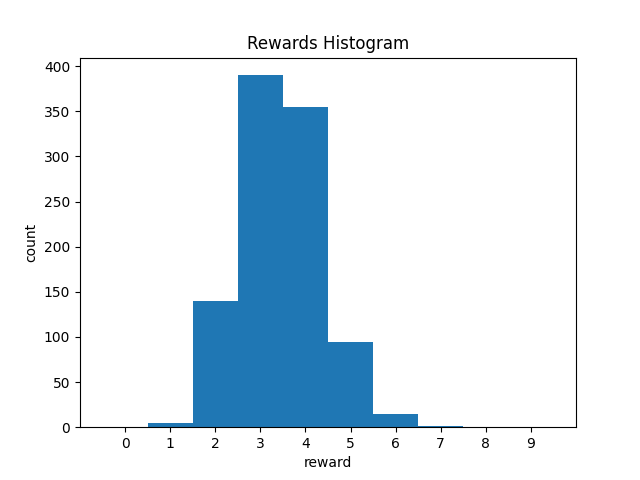
\includegraphics[width=\textwidth]{fig/asg1_reward_hist.png}
        \caption{rewards histogram over 1000 runs}
        \label{fig:fig_1}
    \end{subfigure}
    \hfill
    \begin{subfigure}[htbp]{0.25\textwidth}
        \centering
        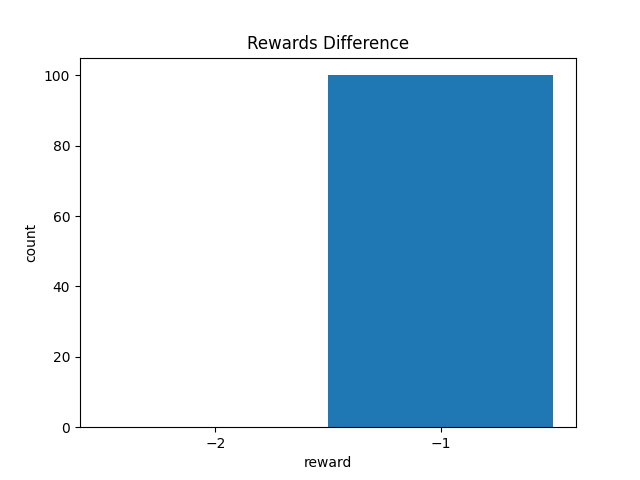
\includegraphics[width=\textwidth]{fig/asg1_reward_diff.png}
        \caption{correctness}
        \label{fig:fig_2}
    \end{subfigure}
    \hfill
    \begin{subfigure}[htbp]{0.25\textwidth}
        \centering
        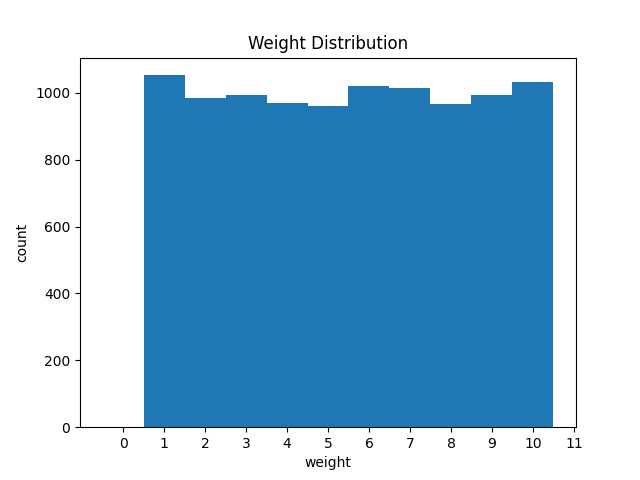
\includegraphics[width=\textwidth]{fig/asg1_weight_dist.png}
        \caption{Item weight distribution}
        \label{fig:weightdist}
    \end{subfigure}
    \hfill
    \begin{subfigure}[htbp]{0.25\textwidth}
        \centering
        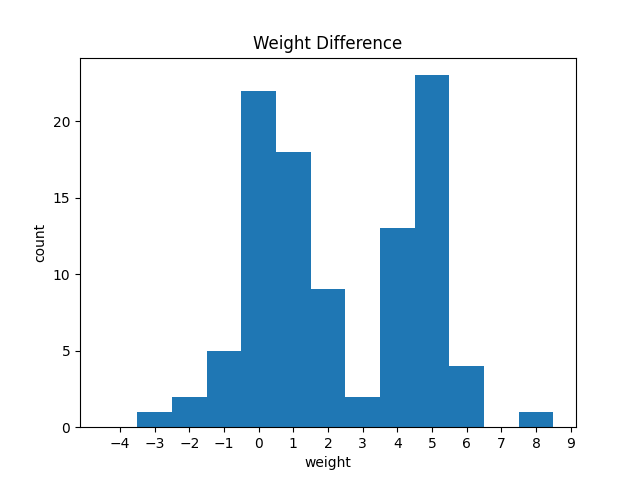
\includegraphics[width=\textwidth]{fig/asg1_weight_diff.png}
        \caption{Leftover weight difference for different reward}
        \label{fig:weightdiff}
    \end{subfigure}
    %\caption {}
    \label{fig:gain}
\end{figure*}
The histogram of the optimal reward is shown in figure \ref{fig:fig_1}, and the average revenue is 3.442, close to the expected optimal, which examines hypothesis 1. Comparing with the deterministic average result of 3.542, the optimal policy can work well. Apart from that, we also discover that the result of the experiment is also influence by the weight distribution and the run times, with 1000 runs, the average result is bigger than the expected optimal, which might mean the distribution of items weights is not strictly align to 0.1 probability, more specifically, with seed 42, the average weight of items is 5.4972. As plotted in figure \ref{fig:weightdist}, the percentage of weight 1 is higher than average which might lead to higher rewards for some of the runs. While scale the experiment runs, this number would getting closer to the optimal expect reward. Prove the effeteness of the algorithm.

Additionally, as plotted in figure \ref{fig:weightdiff}, the two hills might represent the two cases in hypothesis 2.

\section{Conclusion}
In this report, we have presented a thorough introduction to the design of the backward induction method, and how to solve a stochastic finite-horizon dynamic decision problem. Through a comparative analysis of their performance compared with the deterministic result, we have proved that the optimal policy could work well, and the average 
%\newpage
